	\subsection{Output fluxes clustering}

		\subsubsection{K-Means}
			
			As K-Means allows for the number of clusters to be defined, and we know that there are 4 in the original dataset, K-Means is used to find 4 clusters.
			
			\begin{table}[h!]
				\centering
				\begin{tabular}{|c|c|c|}
					\hline
					& \textbf{Number of clusters} & \textbf{Number of initializations}\\
					\hline
					\textbf{Original Output fluxes} & 4 & 10\\
					\hline
					\textbf{PCA Output fluxes} & 4 & 10\\
					\hline
					\textbf{UMAP Output fluxes} & 4 & 10\\
					\hline
				\end{tabular}
				\caption{K-Means hyperparameter configuration for c coefficients clustering}
			\end{table}
		
			The results are the following:
			
			\begin{figure*}[ht!]
				\centering
				\subfloat[Original cluster densities]{%
					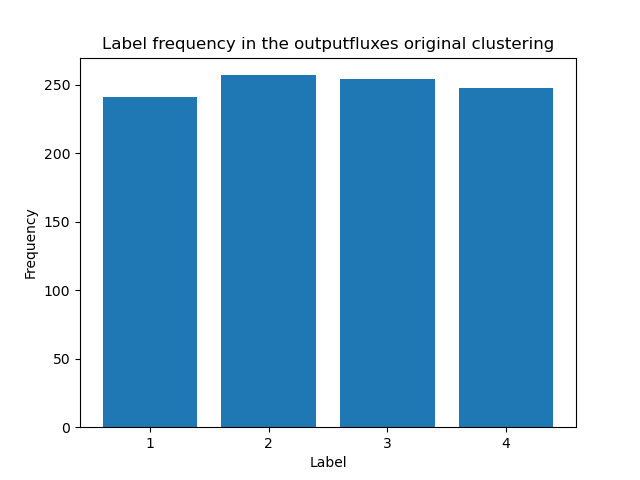
\includegraphics[width=0.45\textwidth]{mdid-outputfluxesoriginaldensity.png}}
				\hspace{\fill}
				\subfloat[K-Means clusters densities]{%
					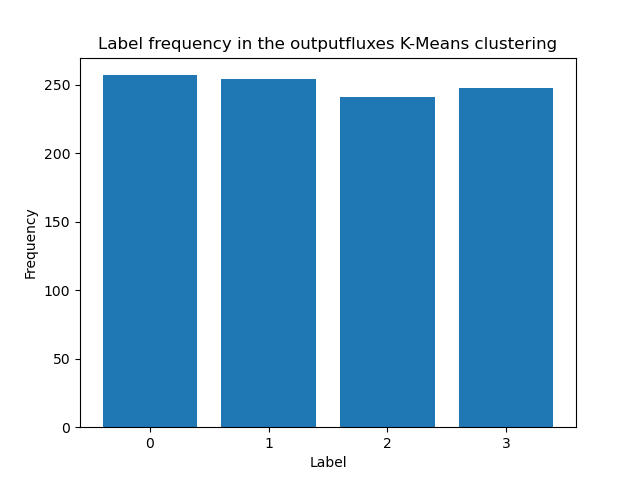
\includegraphics[width=0.45\textwidth]{mdid-outputfluxesK-Meansdensity.png}}\\
				\subfloat[Original clusters]{%
					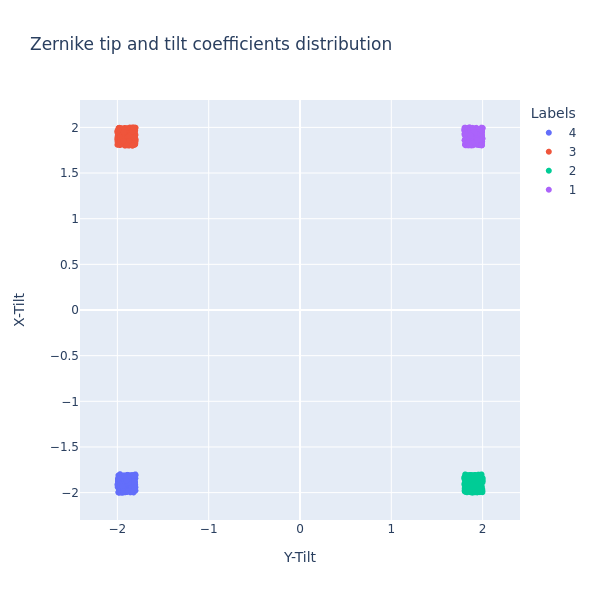
\includegraphics[width=0.45\textwidth]{mdid-originalclusters.png}}
				\hspace{\fill}
				\subfloat[K-Means clusters]{%
					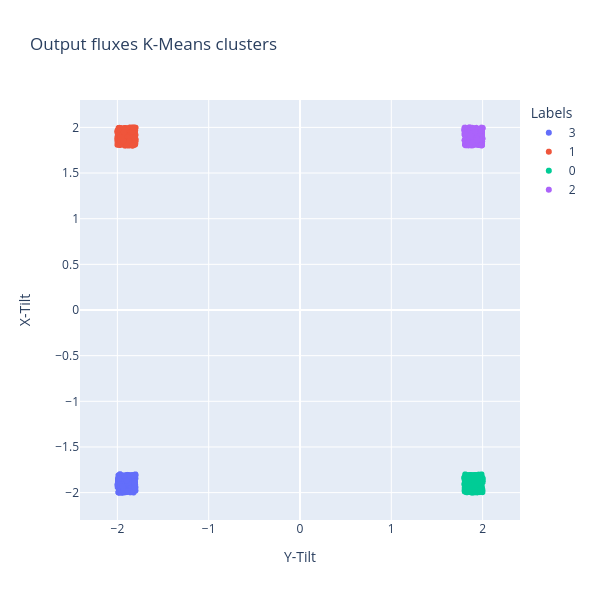
\includegraphics[width=0.45\textwidth]{mdid-outputfluxesK-Meansclusters.png}}\\
					
				\subfloat[Original cluster samples]{%
					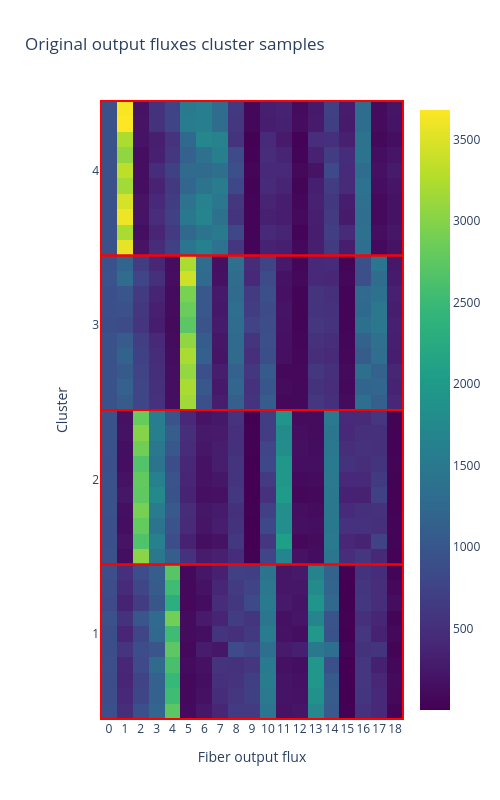
\includegraphics[width=0.4\textwidth]{mdid-outputfluxesoriginalgridclusters.png}}
				\hspace{\fill}
				\subfloat[K-Means cluster samples]{%
					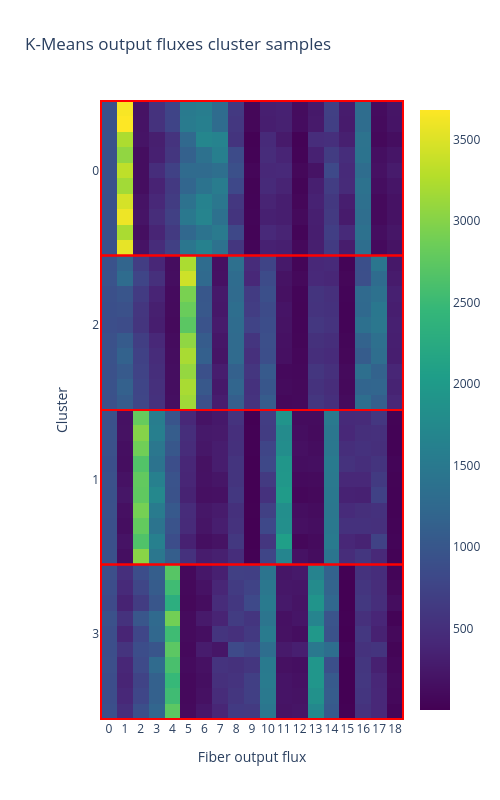
\includegraphics[width=0.4\textwidth]{mdid-outputfluxesK-Meansgridclusters.png}}
				\caption{Comparison between original clustering and K-Means clustering from original Output fluxes}
			\end{figure*}
			\FloatBarrier
		
			\begin{figure*}[ht!]
				\centering
				\subfloat[Original cluster densities from PCA]{%
					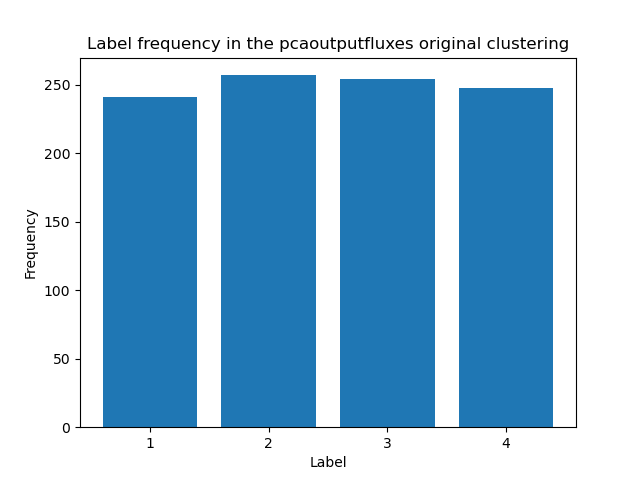
\includegraphics[width=0.45\textwidth]{mdid-pcaoutputfluxesoriginaldensity.png}}
				\hspace{\fill}
				\subfloat[K-Means clusters densities from PCA]{%
					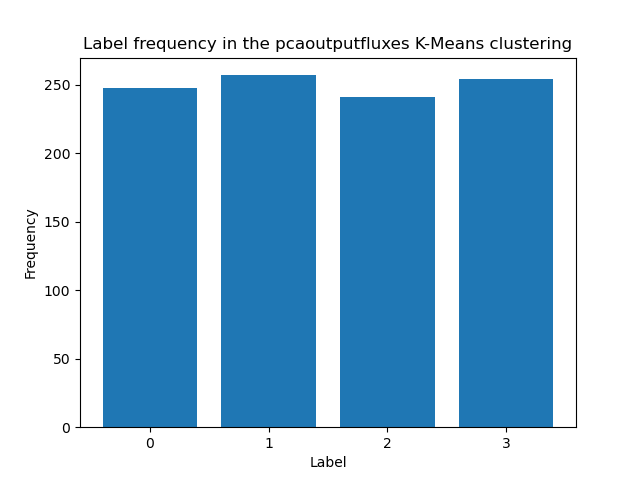
\includegraphics[width=0.45\textwidth]{mdid-pcaoutputfluxesK-Meansdensity.png}}\\
				\subfloat[Original clusters]{%
					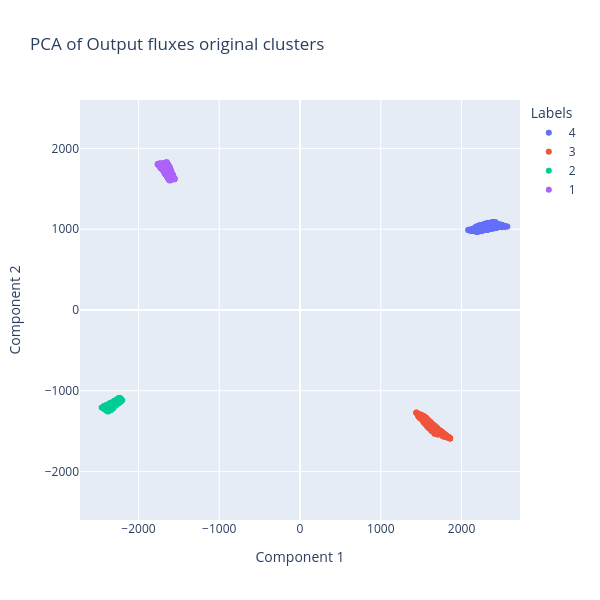
\includegraphics[width=0.45\textwidth]{mdid-pcaoutputfluxesoriginalclusters.png}}
				\hspace{\fill}
				\subfloat[K-Means clusters from PCA]{%
					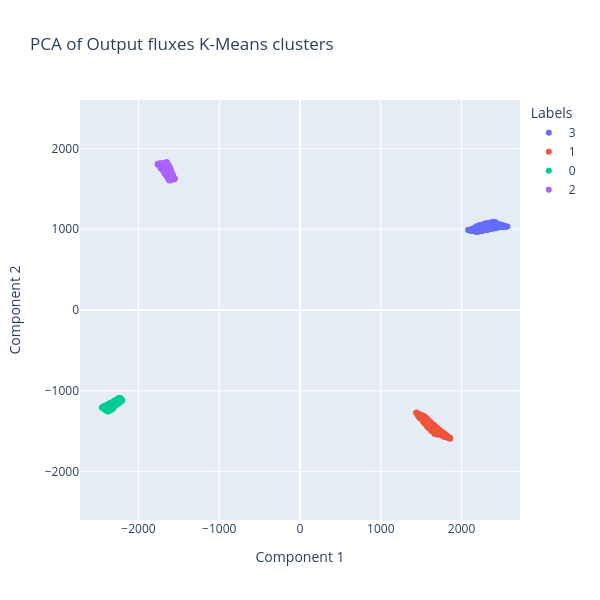
\includegraphics[width=0.45\textwidth]{mdid-pcaoutputfluxesK-Meansclusters.png}}\\
					
				\subfloat[Original cluster samples from PCA]{%
					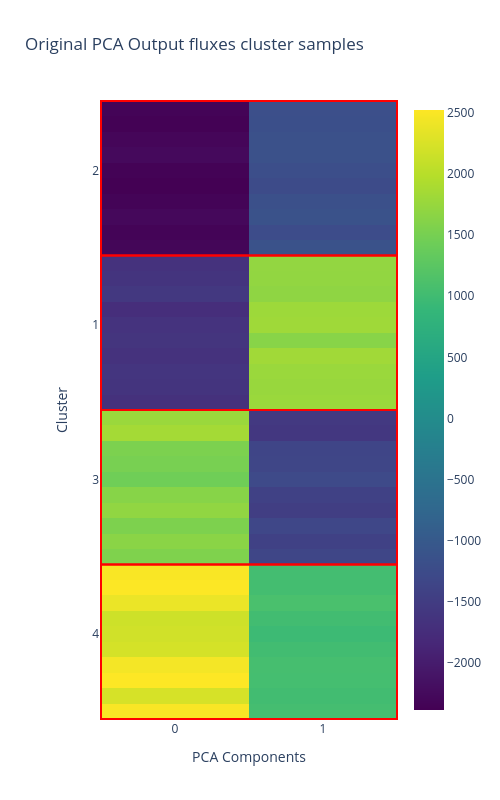
\includegraphics[width=0.4\textwidth]{mdid-pcaoutputfluxesoriginalgridclusters.png}}
				\hspace{\fill}
				\subfloat[K-Means cluster samples from PCA]{%
					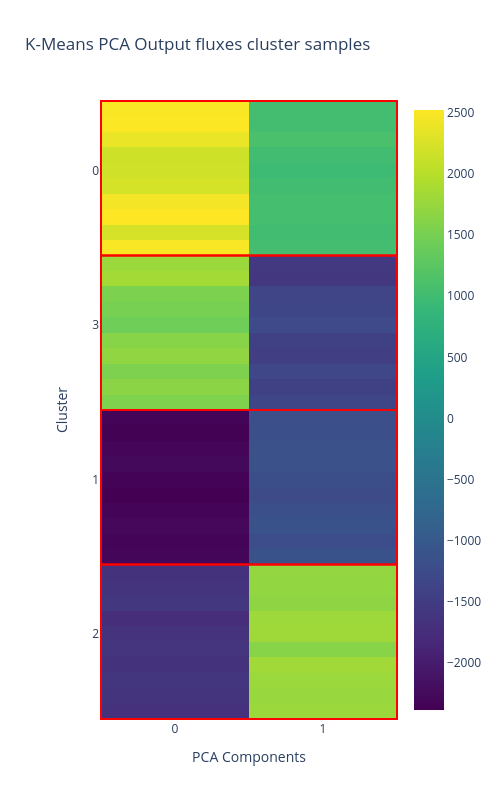
\includegraphics[width=0.4\textwidth]{mdid-pcaoutputfluxesK-Meansgridclusters.png}}
				\caption{Comparison between original clustering and K-Means clustering from PCA of Output fluxes}
			\end{figure*}
			\FloatBarrier
			
			\begin{figure*}[ht!]
				\centering
				\subfloat[Original cluster densities from UMAP]{%
					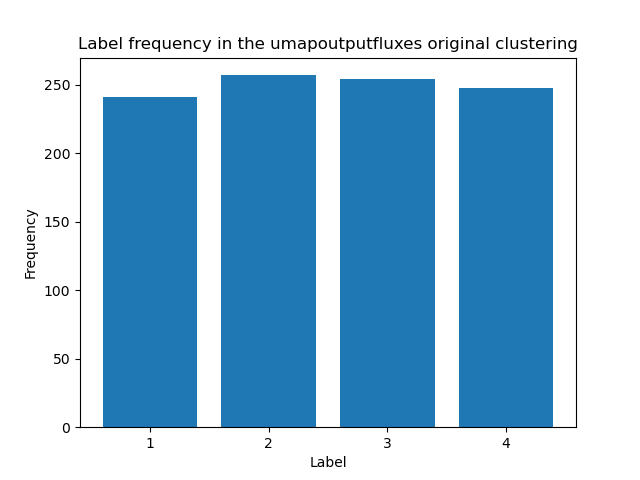
\includegraphics[width=0.45\textwidth]{mdid-umapoutputfluxesoriginaldensity.png}}
				\hspace{\fill}
				\subfloat[K-Means clusters densities from UMAP]{%
					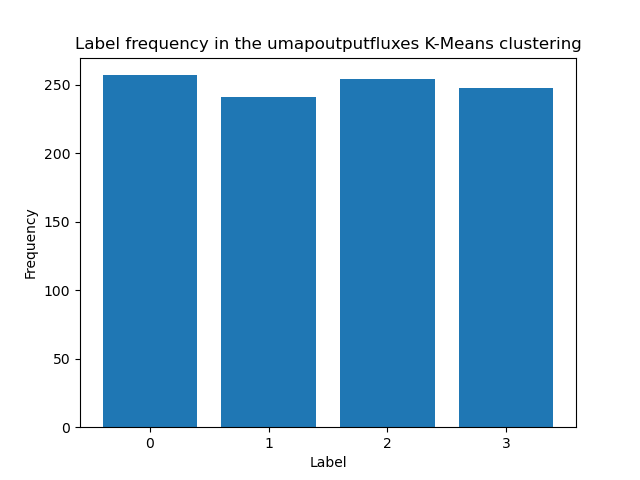
\includegraphics[width=0.45\textwidth]{mdid-umapoutputfluxesK-Meansdensity.png}}\\
				\subfloat[Original clusters from UMAP]{%
					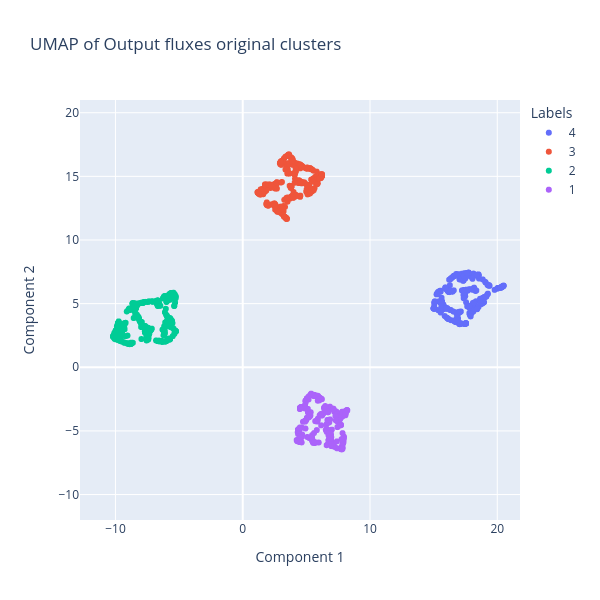
\includegraphics[width=0.45\textwidth]{mdid-umapoutputfluxesoriginalclusters.png}}
				\hspace{\fill}
				\subfloat[K-Means clusters from UMAP]{%
					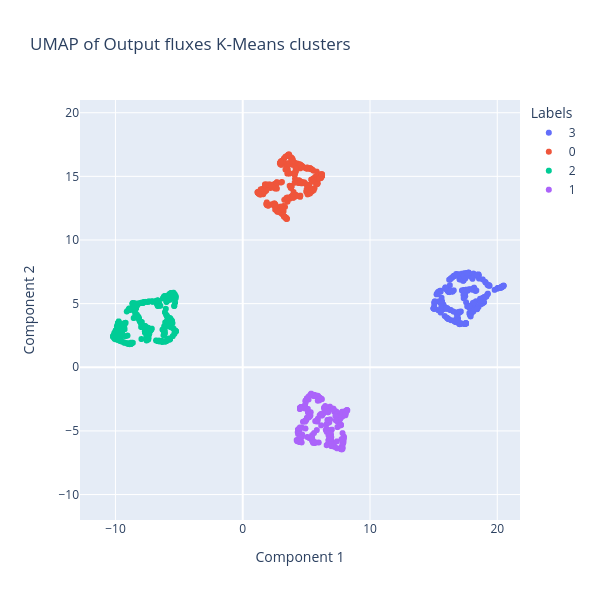
\includegraphics[width=0.45\textwidth]{mdid-umapoutputfluxesK-Meansclusters.png}}\\
					
				\subfloat[Original cluster samples from UMAP]{%
					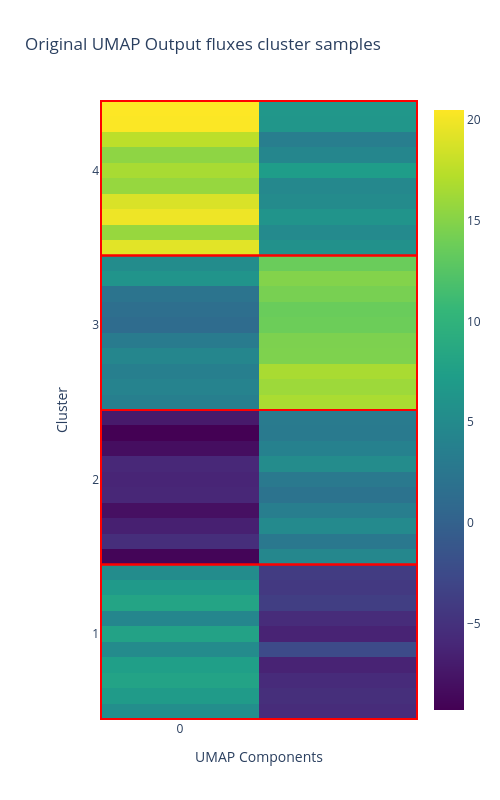
\includegraphics[width=0.4\textwidth]{mdid-umapoutputfluxesoriginalgridclusters.png}}
				\hspace{\fill}
				\subfloat[K-Means cluster samples from UMAP]{%
					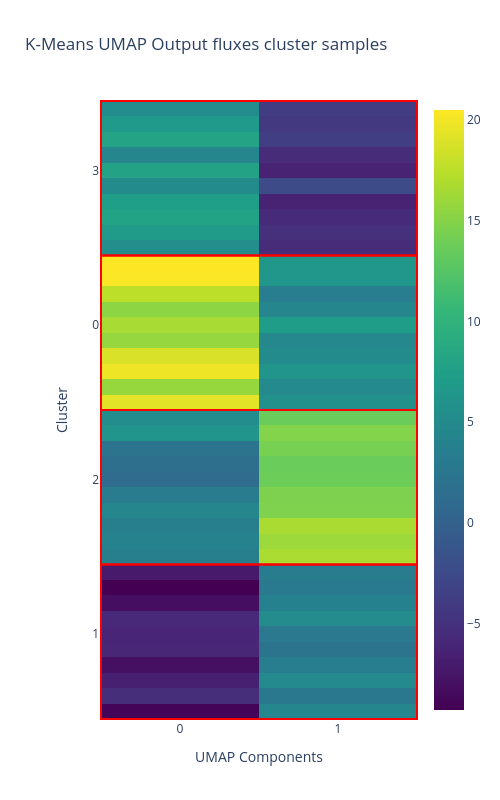
\includegraphics[width=0.4\textwidth]{mdid-umapoutputfluxesK-Meansgridclusters.png}}
				\caption{Comparison between original clustering and K-Means clustering from UMAP of Output fluxes}
			\end{figure*}
			\FloatBarrier
		
		\subsubsection{DBSCAN}
			
			A configuration that outputs 4 clusters is searched
			
			\begin{table}[h!]
				\centering
				\begin{tabular}{|c|c|c|}
					\hline
					& \textbf{Number of neighbours} & \textbf{Epsilon}\\
					\hline
					Original Output fluxes & 7 & 120\\
					\hline
					PCA Output fluxes & 15 & 40\\
					\hline
					UMAP Output fluxes & 10 & 0.85\\
					\hline
				\end{tabular}
				\caption{DBSCAN hyperparameter configuration for Output fluxes clustering}
			\end{table}
		
			The results are the following:
			
			\begin{figure*}[ht!]
				\centering
				\subfloat[Original cluster densities]{%
					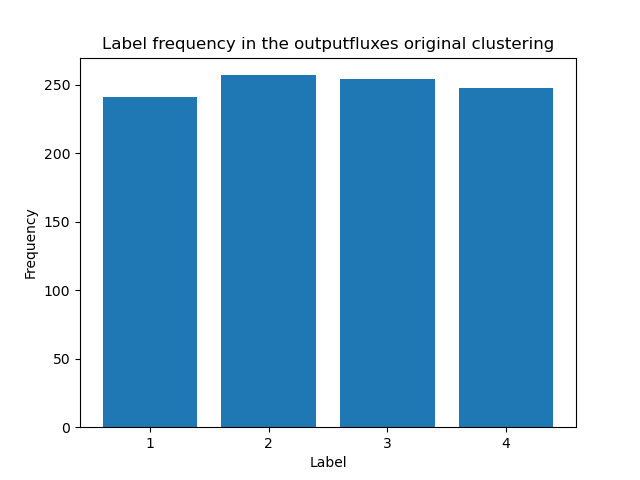
\includegraphics[width=0.45\textwidth]{mdid-outputfluxesoriginaldensity.png}}
				\hspace{\fill}
				\subfloat[DBSCAN clusters densities]{%
					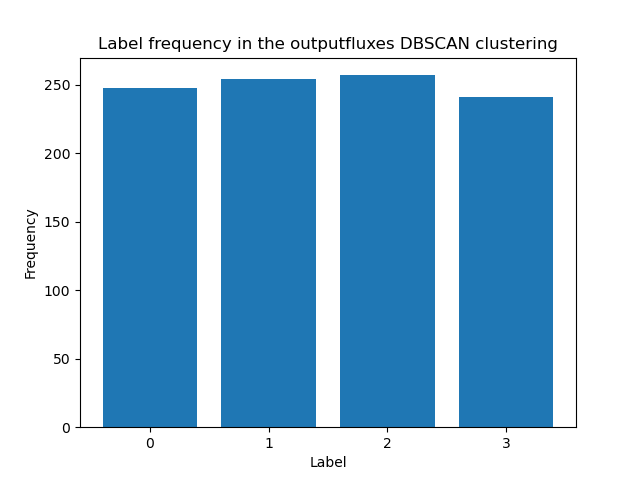
\includegraphics[width=0.45\textwidth]{mdid-outputfluxesDBSCANdensity.png}}
				\\
				\subfloat[Original clusters]{%
					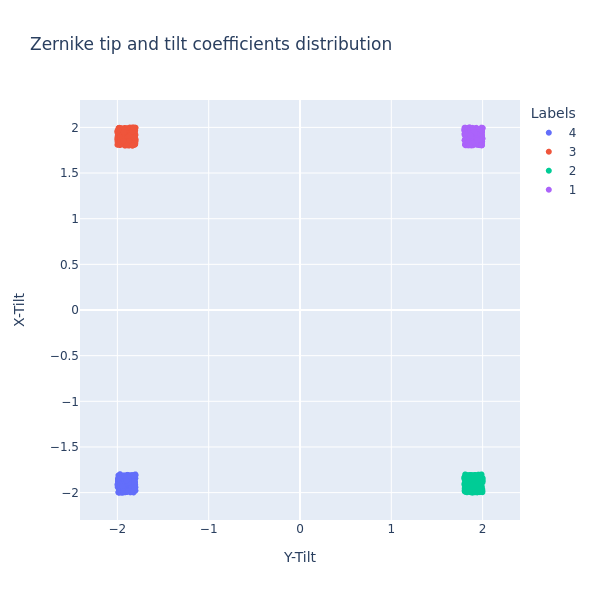
\includegraphics[width=0.45\textwidth]{mdid-originalclusters.png}}
				\hspace{\fill}
				\subfloat[DBSCAN clusters]{%
					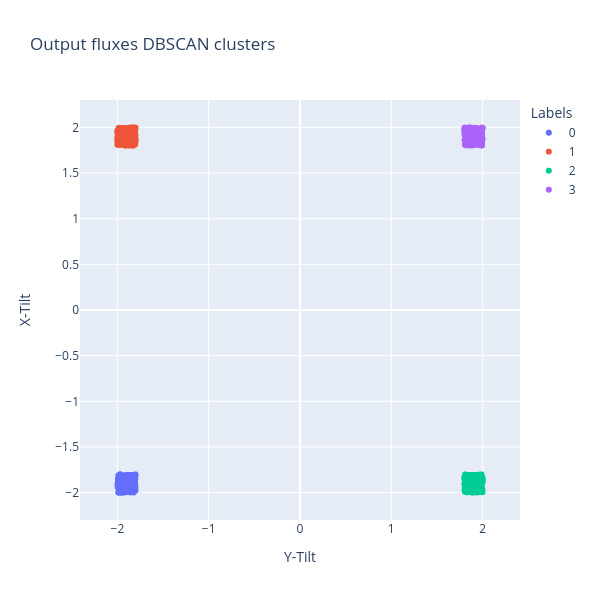
\includegraphics[width=0.45\textwidth]{mdid-outputfluxesDBSCANclusters.png}}\\
					
				\subfloat[Original cluster samples]{%
					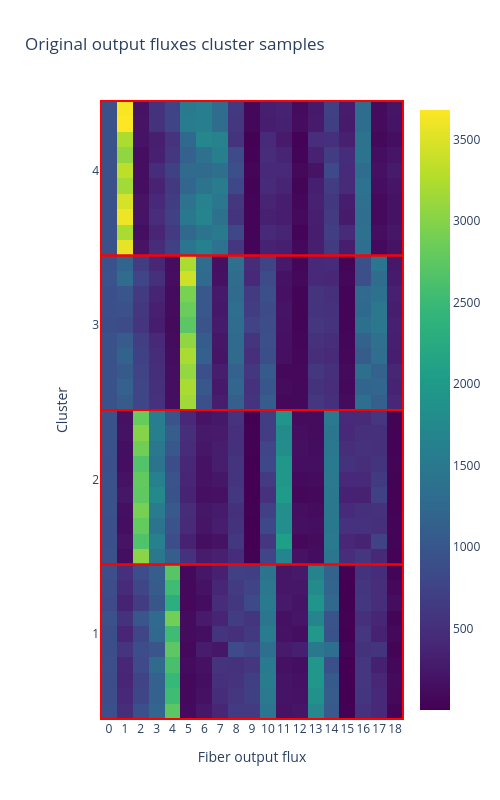
\includegraphics[width=0.4\textwidth]{mdid-outputfluxesoriginalgridclusters.png}}
				\hspace{\fill}
				\subfloat[DBSCAN cluster samples]{%
					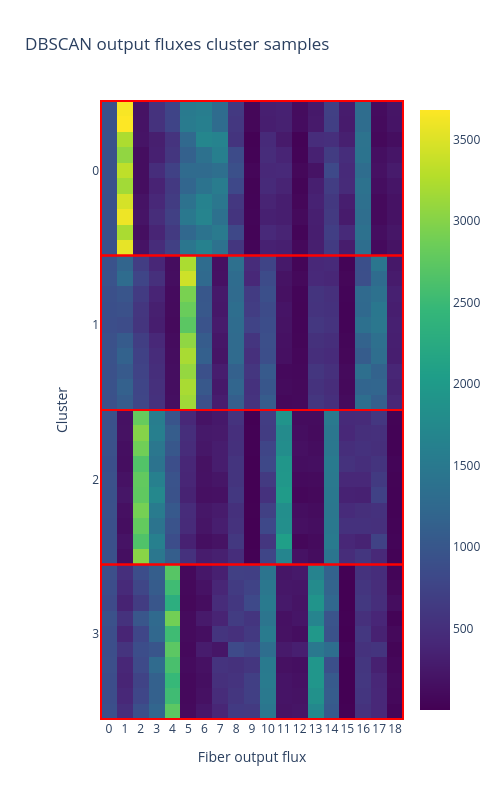
\includegraphics[width=0.4\textwidth]{mdid-outputfluxesDBSCANgridclusters.png}}
				\caption{Comparison between original clustering and DBSCAN clustering}
			\end{figure*}
			\FloatBarrier
			
			\begin{figure*}[ht!]
				\centering
				\subfloat[Original cluster densities from PCA]{%
					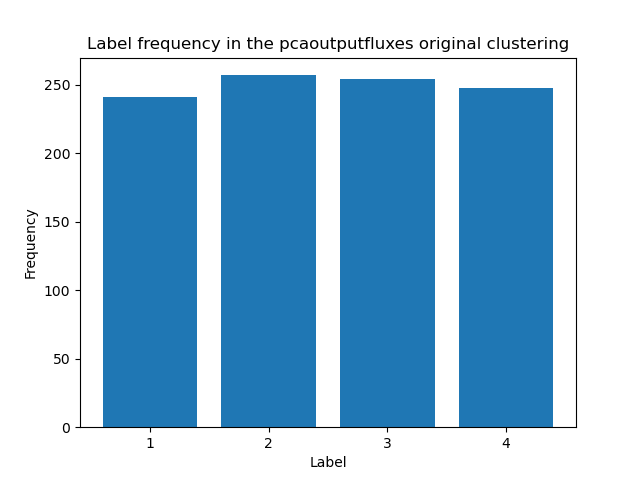
\includegraphics[width=0.45\textwidth]{mdid-pcaoutputfluxesoriginaldensity.png}}
				\hspace{\fill}
				\subfloat[DBSCAN clusters densities from PCA]{%
					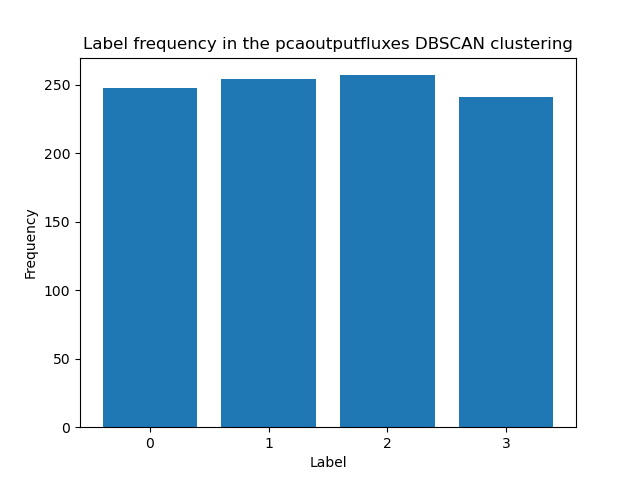
\includegraphics[width=0.45\textwidth]{mdid-pcaoutputfluxesDBSCANdensity.png}}
				\\
				\subfloat[Original clusters from PCA]{%
					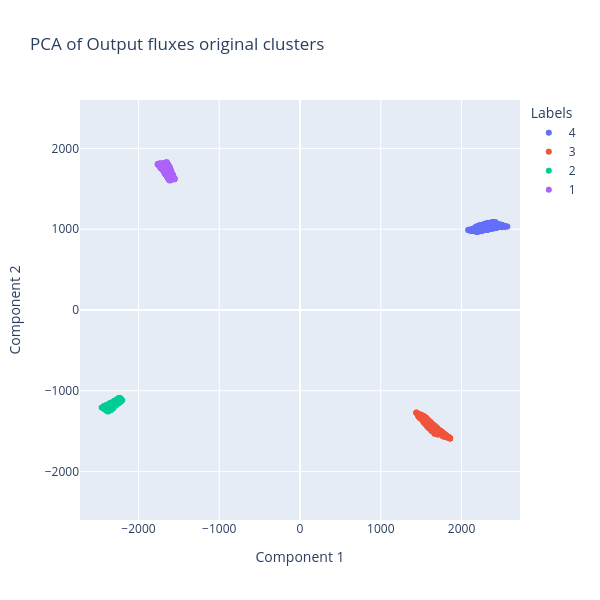
\includegraphics[width=0.45\textwidth]{mdid-pcaoutputfluxesoriginalclusters.png}}
				\hspace{\fill}
				\subfloat[DBSCAN clusters from PCA]{%
					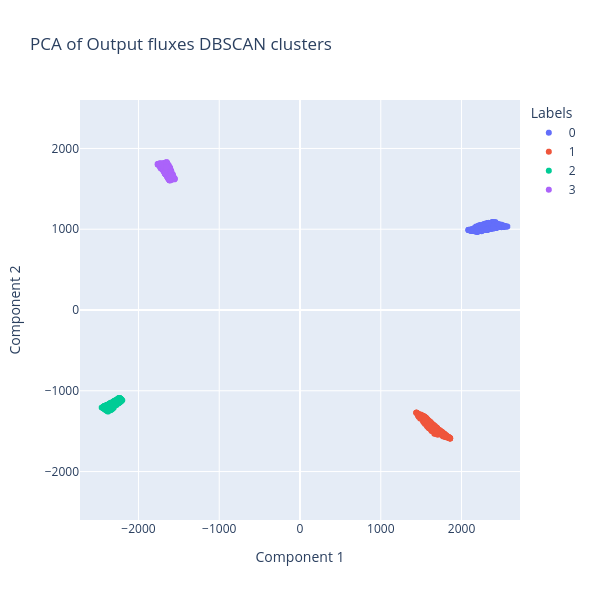
\includegraphics[width=0.45\textwidth]{mdid-pcaoutputfluxesDBSCANclusters.png}}\\
					
				\subfloat[Original cluster samples from PCA]{%
					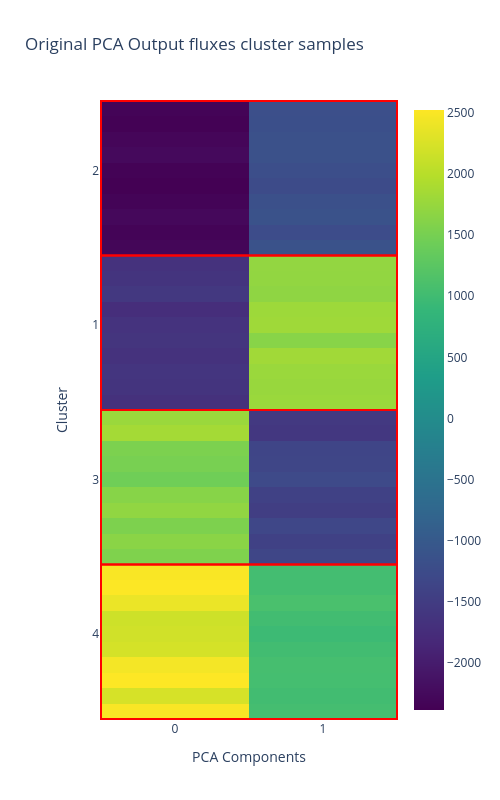
\includegraphics[width=0.4\textwidth]{mdid-pcaoutputfluxesoriginalgridclusters.png}}
				\hspace{\fill}
				\subfloat[DBSCAN cluster samples from PCA]{%
					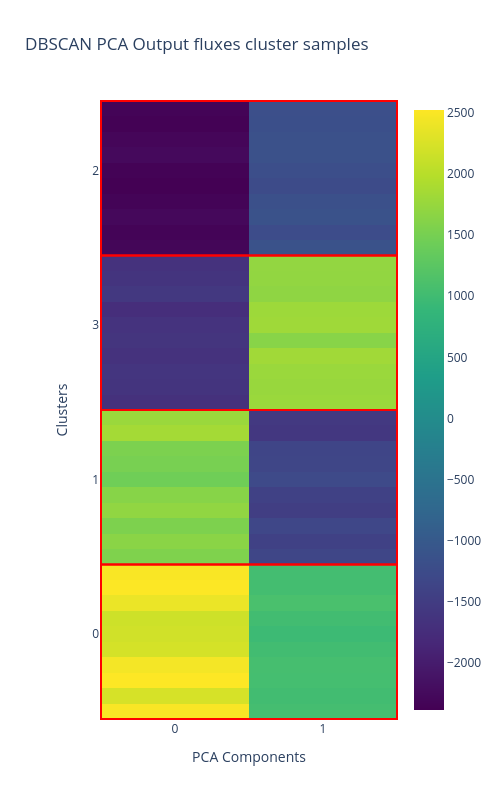
\includegraphics[width=0.4\textwidth]{mdid-pcaoutputfluxesDBSCANgridclusters.png}}
				\caption{Comparison between original clustering and DBSCAN clustering from PCA of Output fluxes}
			\end{figure*}
			\FloatBarrier
			
			\begin{figure*}[ht!]
				\centering
				\subfloat[Original cluster densities from UMAP]{%
					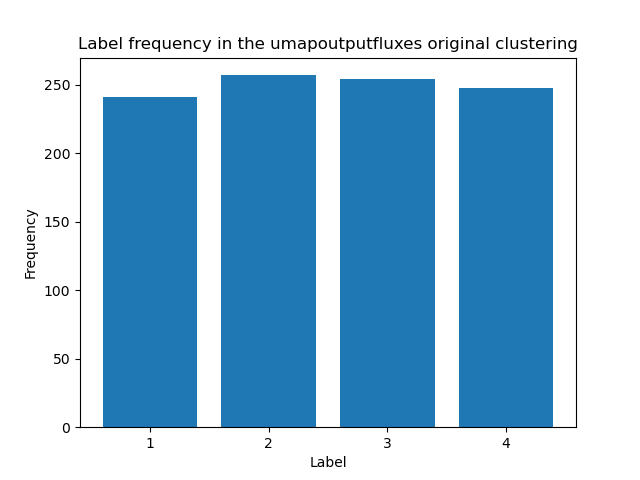
\includegraphics[width=0.45\textwidth]{mdid-umapoutputfluxesoriginaldensity.png}}
				\hspace{\fill}
				\subfloat[DBSCAN clusters densities from UMAP]{%
					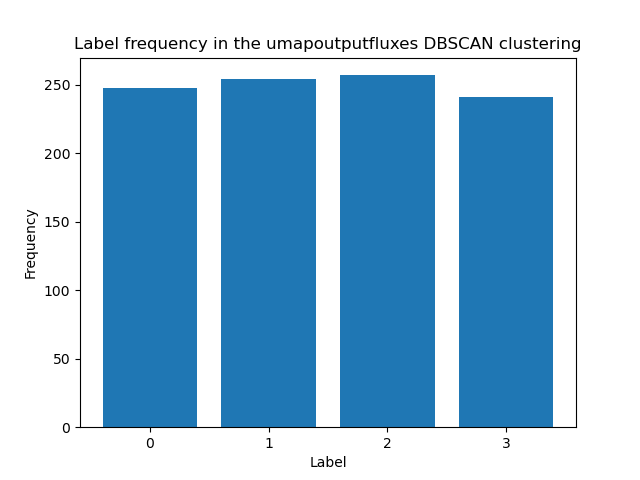
\includegraphics[width=0.45\textwidth]{mdid-umapoutputfluxesDBSCANdensity.png}}\\
				\subfloat[Original clusters from UMAP]{%
					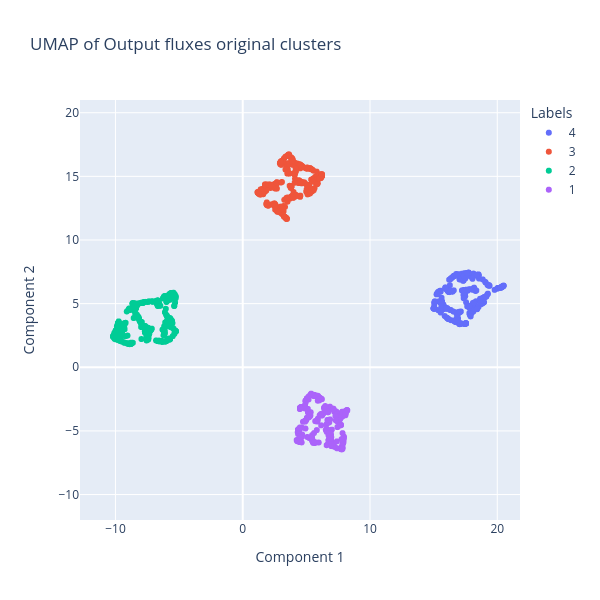
\includegraphics[width=0.45\textwidth]{mdid-umapoutputfluxesoriginalclusters.png}}
				\hspace{\fill}
				\subfloat[DBSCAN clusters from UMAP]{%
					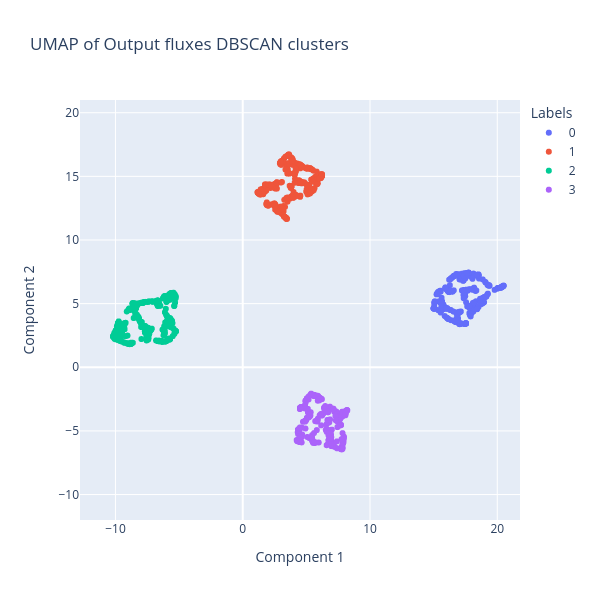
\includegraphics[width=0.45\textwidth]{mdid-umapoutputfluxesDBSCANclusters.png}}\\
					
				\subfloat[Original cluster samples from UMAP]{%
					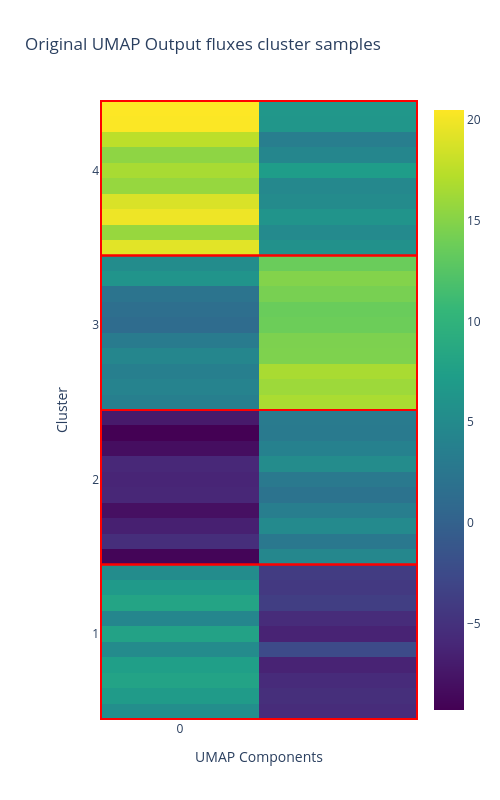
\includegraphics[width=0.4\textwidth]{mdid-umapoutputfluxesoriginalgridclusters.png}}
				\hspace{\fill}
				\subfloat[DBSCAN cluster samples from UMAP]{%
					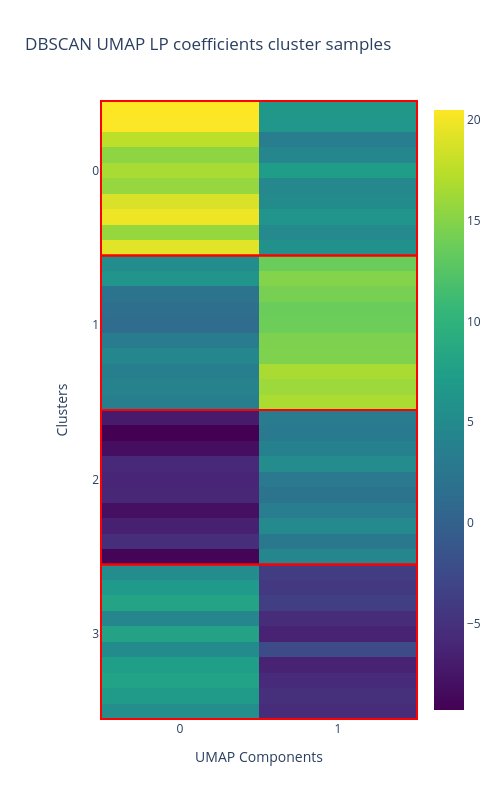
\includegraphics[width=0.4\textwidth]{mdid-umapoutputfluxesDBSCANgridclusters.png}}
				\caption{Comparison between original clustering and DBSCAN clustering from UMAP of Output fluxes}
			\end{figure*}
			\FloatBarrier
		
		\subsubsection{HDBSCAN}
			
			A configuration that outputs 4 clusters is searched.
			
			\begin{table}[h!]
				\centering
				\begin{tabular}{|c|c|c|}
					\hline
					& \textbf{Minimum cluster size} \\
					\hline
					Original Output fluxes & 21 \\
					\hline
					PCA Output fluxes & 21 \\
					\hline
					HDBSCAN Output fluxes & 25 \\
					\hline
				\end{tabular}
				\caption{HDBSCAN hyperparameter configuration for Output fluxes clustering}
			\end{table}
			\FloatBarrier
			
			The results are the following:
			
			\begin{figure*}[ht!]
				\centering
				\subfloat[Original cluster densities]{%
					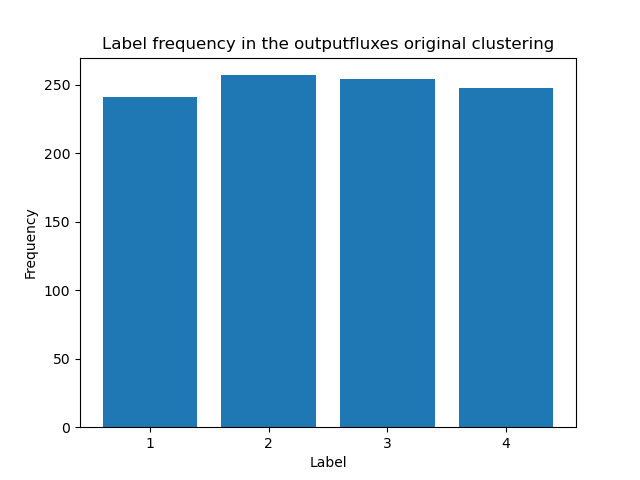
\includegraphics[width=0.45\textwidth]{mdid-outputfluxesoriginaldensity.png}}
				\hspace{\fill}
				\subfloat[HDBSCAN clusters densities]{%
					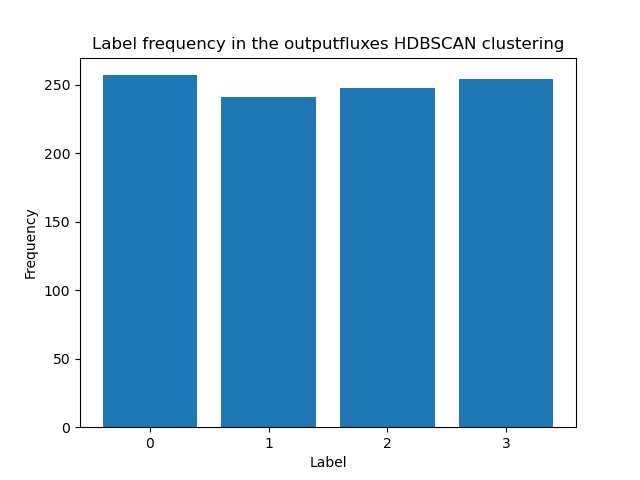
\includegraphics[width=0.45\textwidth]{mdid-outputfluxesHDBSCANdensity.png}}
				\\
				\subfloat[Original clusters]{%
					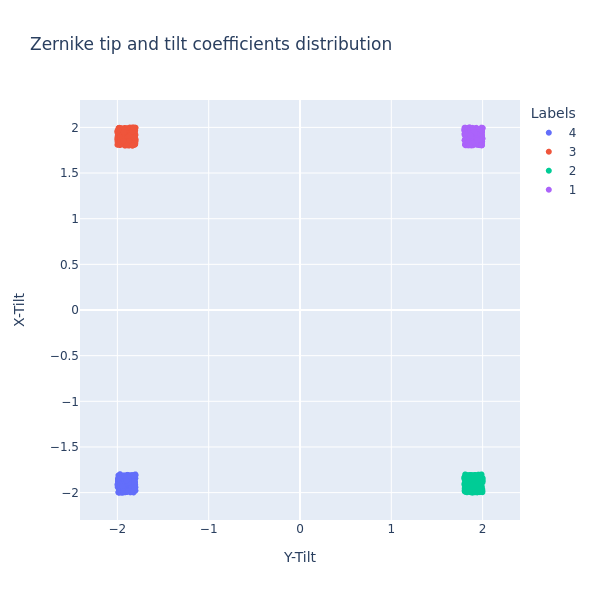
\includegraphics[width=0.45\textwidth]{mdid-originalclusters.png}}
				\hspace{\fill}
				\subfloat[HDBSCAN clusters]{%
					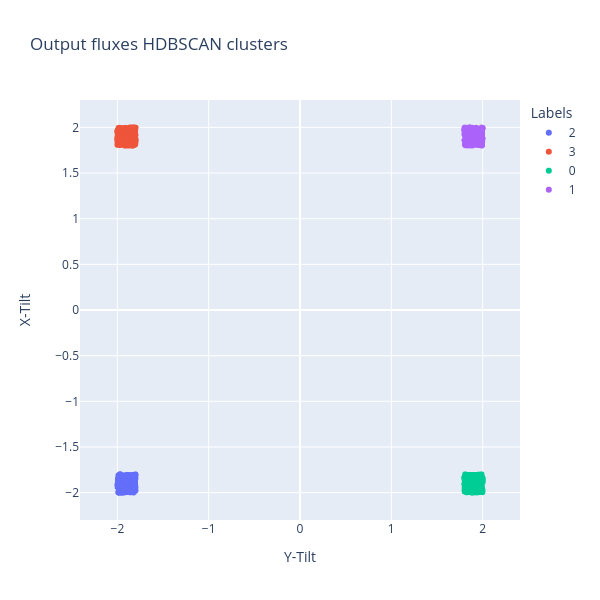
\includegraphics[width=0.45\textwidth]{mdid-outputfluxesHDBSCANclusters.png}}\\
					
				\subfloat[Original cluster samples]{%
					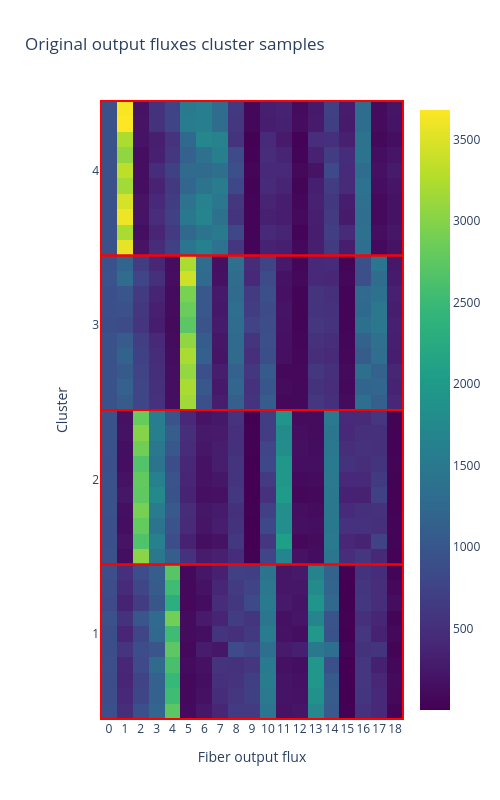
\includegraphics[width=0.4\textwidth]{mdid-outputfluxesoriginalgridclusters.png}}
				\hspace{\fill}
				\subfloat[HDBSCAN cluster samples]{%
					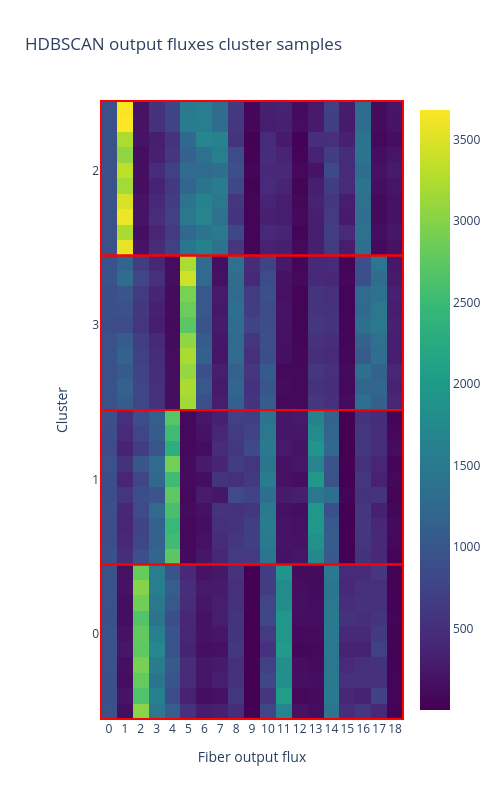
\includegraphics[width=0.4\textwidth]{mdid-outputfluxesHDBSCANgridclusters.png}}
				\caption{Comparison between original clustering and HDBSCAN clustering}
			\end{figure*}
			\FloatBarrier
			
			\begin{figure*}[ht!]
				\centering
				\subfloat[Original cluster densities from PCA]{%
					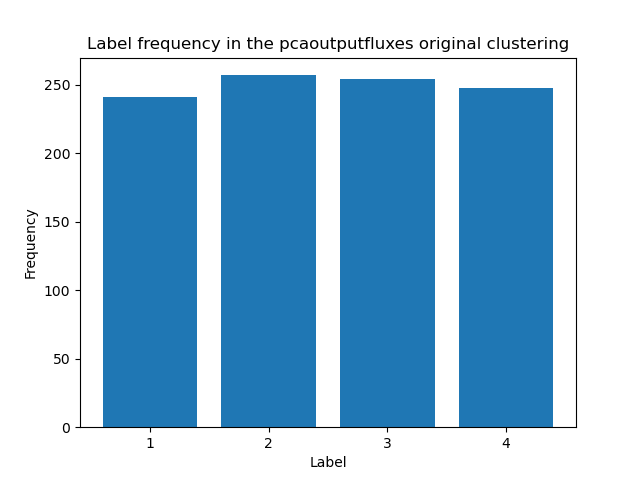
\includegraphics[width=0.45\textwidth]{mdid-pcaoutputfluxesoriginaldensity.png}}
				\hspace{\fill}
				\subfloat[HDBSCAN clusters densities from PCA]{%
					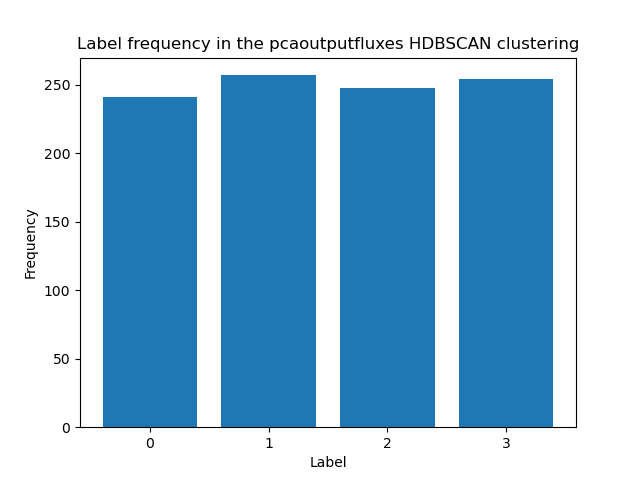
\includegraphics[width=0.45\textwidth]{mdid-pcaoutputfluxesHDBSCANdensity.png}}
				\\
				\subfloat[Original clusters from PCA]{%
					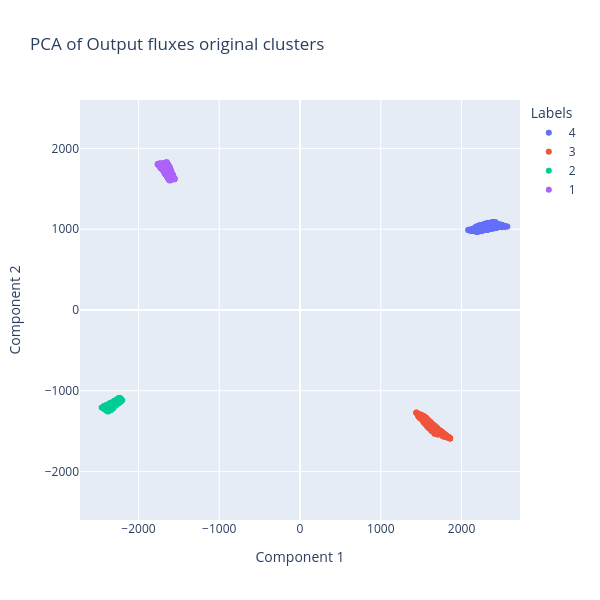
\includegraphics[width=0.45\textwidth]{mdid-pcaoutputfluxesoriginalclusters.png}}
				\hspace{\fill}
				\subfloat[HDBSCAN clusters from PCA]{%
					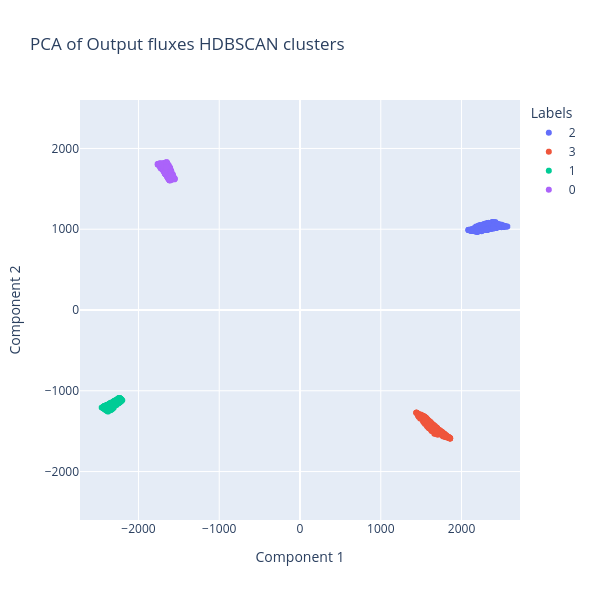
\includegraphics[width=0.45\textwidth]{mdid-pcaoutputfluxesHDBSCANclusters.png}}\\
					
				\subfloat[Original cluster samples from PCA]{%
					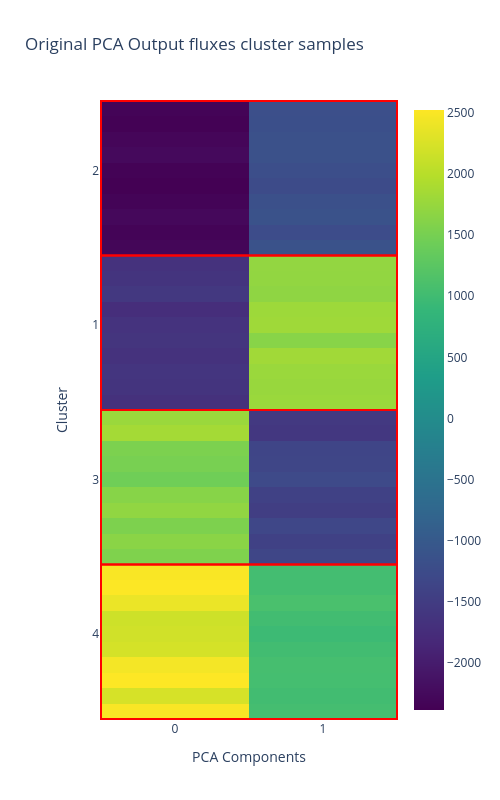
\includegraphics[width=0.4\textwidth]{mdid-pcaoutputfluxesoriginalgridclusters.png}}
				\hspace{\fill}
				\subfloat[HDBSCAN cluster samples from PCA]{%
					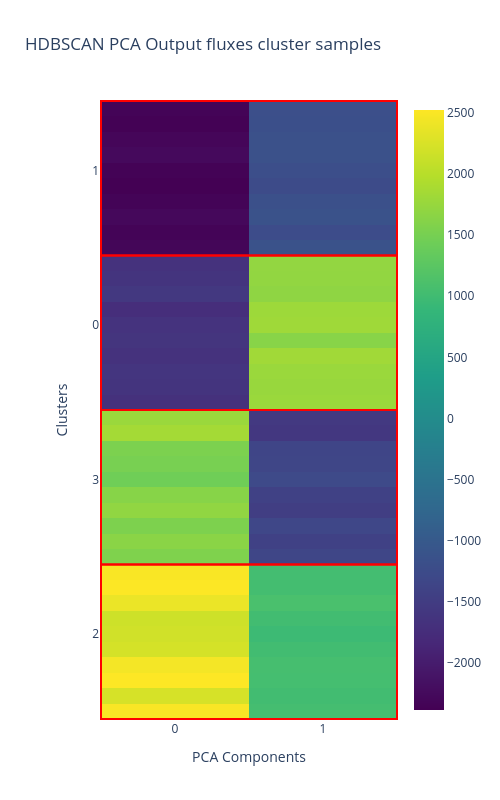
\includegraphics[width=0.4\textwidth]{mdid-pcaoutputfluxesHDBSCANgridclusters.png}}
				\caption{Comparison between original clustering and HDBSCAN clustering from PCA of Output fluxes}
			\end{figure*}
			\FloatBarrier
			
			\begin{figure*}[ht!]
				\centering
				\subfloat[Original cluster densities from UMAP]{%
					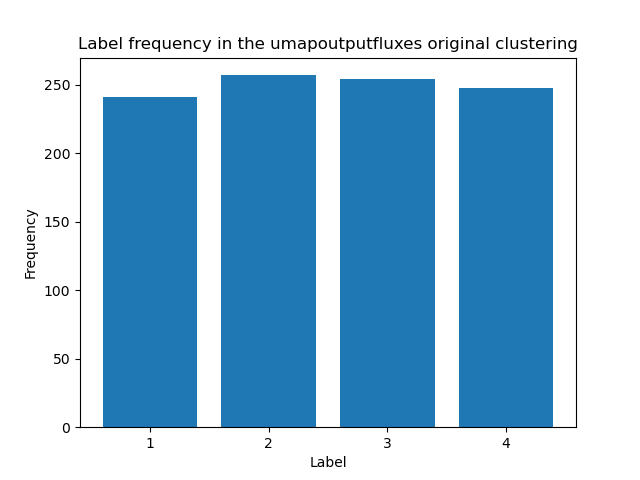
\includegraphics[width=0.45\textwidth]{mdid-umapoutputfluxesoriginaldensity.png}}
				\hspace{\fill}
				\subfloat[HDBSCAN clusters densities from UMAP]{%
					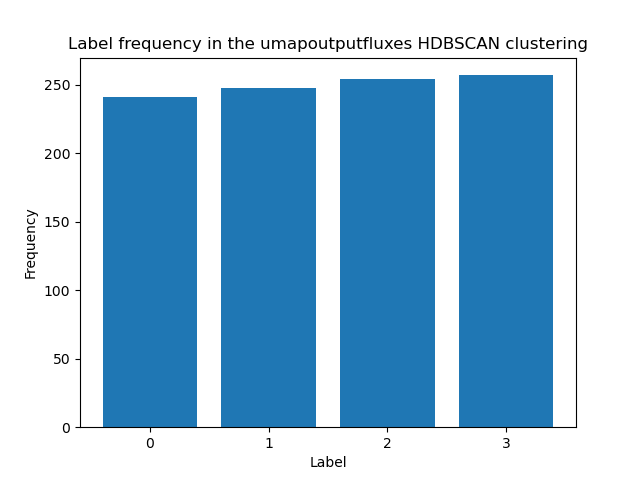
\includegraphics[width=0.45\textwidth]{mdid-umapoutputfluxesHDBSCANdensity.png}}\\
				\subfloat[Original clusters from UMAP]{%
					\includegraphics[width=0.45\textwidth]{mdid-umapoutputfluxesoriginalclusters.png}}
				\hspace{\fill}
				\subfloat[HDBSCAN clusters from UMAP]{%
					\includegraphics[width=0.45\textwidth]{mdid-umapoutputfluxesHDBSCANclusters.png}}\\
					
				\subfloat[Original cluster samples from UMAP]{%
					\includegraphics[width=0.4\textwidth]{mdid-umapoutputfluxesoriginalgridclusters.png}}
				\hspace{\fill}
				\subfloat[HDBSCAN cluster samples from UMAP]{%
					\includegraphics[width=0.4\textwidth]{mdid-umapoutputfluxesHDBSCANgridclusters.png}}
				\caption{Comparison between original clustering and HDBSCAN clustering from UMAP of Output fluxes}
			\end{figure*}
			\FloatBarrier
		
		\subsubsection{Agglomerative clustering}
			\begin{table}[h!]
				\centering
				\begin{tabular}{|c|c|}
					\hline
					 & \textbf{Number of clusters} \\
					\hline
					Original Output fluxes & 4 \\
					\hline
					PCA Output fluxes & 4 \\
					\hline
					UMAP Output fluxes & 4 \\
					\hline
				\end{tabular}
				\caption{Agglomerative hyperparameter configuration for Output fluxes clustering}
			\end{table}
			\FloatBarrier
			The results are the following:
			
			\begin{figure*}[ht!]
				\centering
				\subfloat[Original cluster densities]{%
					\includegraphics[width=0.45\textwidth]{mdid-outputfluxesoriginaldensity.png}}
				\hspace{\fill}
				\subfloat[Agglomerative clusters densities]{%
					\includegraphics[width=0.45\textwidth]{mdid-outputfluxesAgglomerativedensity.png}}
				\\
				\subfloat[Original clusters]{%
					\includegraphics[width=0.45\textwidth]{mdid-originalclusters.png}}
				\hspace{\fill}
				\subfloat[Agglomerative clusters]{%
					\includegraphics[width=0.45\textwidth]{mdid-outputfluxesAgglomerativeclusters.png}}\\
					
				\subfloat[Original cluster samples]{%
					\includegraphics[width=0.4\textwidth]{mdid-outputfluxesoriginalgridclusters.png}}
				\hspace{\fill}
				\subfloat[Agglomerative cluster samples]{%
					\includegraphics[width=0.4\textwidth]{mdid-outputfluxesAgglomerativegridclusters.png}}
				\caption{Comparison between original clustering and Agglomerative clustering}
			\end{figure*}
			\FloatBarrier
			
			\begin{figure*}[ht!]
				\centering
				\subfloat[Original cluster densities from PCA]{%
					\includegraphics[width=0.45\textwidth]{mdid-pcaoutputfluxesoriginaldensity.png}}
				\hspace{\fill}
				\subfloat[Agglomerative clusters densities from PCA]{%
					\includegraphics[width=0.45\textwidth]{mdid-pcaoutputfluxesAgglomerativedensity.png}}
				\\
				\subfloat[Original clusters from PCA]{%
					\includegraphics[width=0.45\textwidth]{mdid-pcaoutputfluxesoriginalclusters.png}}
				\hspace{\fill}
				\subfloat[Agglomerative clusters from PCA]{%
					\includegraphics[width=0.45\textwidth]{mdid-pcaoutputfluxesAgglomerativeclusters.png}}\\
					
				\subfloat[Original cluster samples from PCA]{%
					\includegraphics[width=0.4\textwidth]{mdid-pcaoutputfluxesoriginalgridclusters.png}}
				\hspace{\fill}
				\subfloat[Agglomerative cluster samples from PCA]{%
					\includegraphics[width=0.4\textwidth]{mdid-pcaoutputfluxesAgglomerativegridclusters.png}}
				\caption{Comparison between original clustering and Agglomerative clustering}
			\end{figure*}
			\FloatBarrier
			
			\begin{figure*}[ht!]
				\centering
				\subfloat[Original cluster densities from UMAP]{%
					\includegraphics[width=0.45\textwidth]{mdid-umapoutputfluxesoriginaldensity.png}}
				\hspace{\fill}
				\subfloat[Agglomerative clusters densities from UMAP]{%
					\includegraphics[width=0.45\textwidth]{mdid-umapoutputfluxesAgglomerativedensity.png}}\\
				\subfloat[Original clusters from UMAP]{%
					\includegraphics[width=0.45\textwidth]{mdid-umapoutputfluxesoriginalclusters.png}}
				\hspace{\fill}
				\subfloat[Agglomerative clusters from UMAP]{%
					\includegraphics[width=0.45\textwidth]{mdid-umapoutputfluxesAgglomerativeclusters.png}}\\
					
				\subfloat[Original cluster samples from UMAP]{%
					\includegraphics[width=0.4\textwidth]{mdid-umapoutputfluxesoriginalgridclusters.png}}
				\hspace{\fill}
				\subfloat[Agglomerative cluster samples from UMAP]{%
					\includegraphics[width=0.4\textwidth]{mdid-umapoutputfluxesAgglomerativegridclusters.png}}
				\caption{Comparison between original clustering and Agglomerative clustering from UMAP of Output fluxes}
			\end{figure*}
			\FloatBarrier
		
		\subsection{Summary}
			\begin{figure*}[ht!]
				\centering
				\subfloat[Original cluster densities]{%
					\includegraphics[width=0.18\textwidth]{mdid-outputfluxesoriginaldensity.png}}
				\hspace{\fill}
				\subfloat[K-means cluster densities]{%
					\includegraphics[width=0.18\textwidth]{mdid-outputfluxesK-Meansdensity.png}}
				\hspace{\fill}
				\subfloat[DBSCAN cluster densities]{%
					\includegraphics[width=0.18\textwidth]{mdid-outputfluxesDBSCANdensity.png}}
				\hspace{\fill}
				\subfloat[HDBSCAN cluster densities]{%
					\includegraphics[width=0.18\textwidth]{mdid-outputfluxesHDBSCANdensity.png}}
				\hspace{\fill}
				\subfloat[Agglomerative cluster densities]{%
					\includegraphics[width=0.18\textwidth]{mdid-outputfluxesAgglomerativedensity.png}}
				\\
				
				\subfloat[Original cluster]{%
					\includegraphics[width=0.18\textwidth]{mdid-originalclusters.png}}
				\hspace{\fill}
				\subfloat[K-means clusters]{%
					\includegraphics[width=0.18\textwidth]{mdid-outputfluxesK-Meansclusters.png}}
				\hspace{\fill}
				\subfloat[DBSCAN cluster clusters]{%
					\includegraphics[width=0.18\textwidth]{mdid-outputfluxesDBSCANclusters.png}}
				\hspace{\fill}
				\subfloat[HDBSCAN clusters]{%
					\includegraphics[width=0.18\textwidth]{mdid-outputfluxesHDBSCANclusters.png}}
				\hspace{\fill}
				\subfloat[Agglomerative clusters]{%
					\includegraphics[width=0.18\textwidth]{mdid-outputfluxesAgglomerativeclusters.png}}\\
				
				\subfloat[Original cluster samples]{%
					\includegraphics[width=0.18\textwidth]{mdid-outputfluxesoriginalgridclusters.png}}
				\hspace{\fill}
				\subfloat[K-means cluster samples]{%
					\includegraphics[width=0.18\textwidth]{mdid-outputfluxesK-Meansgridclusters.png}}
				\hspace{\fill}
				\subfloat[DBSCAN cluster samples]{%
					\includegraphics[width=0.18\textwidth]{mdid-outputfluxesDBSCANgridclusters.png}}
				\hspace{\fill}
				\subfloat[HDBSCAN cluster samples]{%
					\includegraphics[width=0.18\textwidth]{mdid-outputfluxesHDBSCANgridclusters.png}}
				\hspace{\fill}
				\subfloat[Agglomerative cluster samples]{%
					\includegraphics[width=0.18\textwidth]{mdid-outputfluxesAgglomerativegridclusters.png}}
				
				\caption{Comparison between clustering Output fluxes algorithms}
			\end{figure*}
		\FloatBarrier
		
		\begin{table}[h!]
    			\centering
    			\begin{tabular}{|c|c|c|c|c|c|}
        			\hline
        			& \textbf{Original} & \textbf{K-Means} & \textbf{DBSCAN} & \textbf{HDBSCAN} & \textbf{Agglomerative} \\
        			\hline
        			\textbf{Original} & \diagbox{}{} & 1 & 1 & 1 & 1 \\
       			\hline
        			\textbf{K-Means} &  & \diagbox{}{} & 1 & 1 & 1\\
        			\hline
        			\textbf{DBSCAN} &  &  & \diagbox{}{} & 1 & 1\\
        			\hline
        			\textbf{HDBSCAN} &  &  &  & \diagbox{}{} & 1\\
       			\hline
    			\end{tabular}
    			\caption{Normalized Mutual Information between original Output fluxes clusters}
		\end{table}
		
		\begin{figure*}[ht!]
				\centering
				\subfloat[Original cluster densities from PCA]{%
					\includegraphics[width=0.18\textwidth]{mdid-pcaoutputfluxesoriginaldensity.png}}
				\hspace{\fill}
				\subfloat[K-means cluster densities from PCA]{%
					\includegraphics[width=0.18\textwidth]{mdid-pcaoutputfluxesK-Meansdensity.png}}
				\hspace{\fill}
				\subfloat[DBSCAN cluster densities from PCA]{%
					\includegraphics[width=0.18\textwidth]{mdid-pcaoutputfluxesDBSCANdensity.png}}
				\hspace{\fill}
				\subfloat[HDBSCAN cluster densities from PCA]{%
					\includegraphics[width=0.18\textwidth]{mdid-pcaoutputfluxesHDBSCANdensity.png}}
				\hspace{\fill}
				\subfloat[Agglomerative cluster densities from PCA]{%
					\includegraphics[width=0.18\textwidth]{mdid-pcaoutputfluxesAgglomerativedensity.png}}
				\\
				
				\subfloat[Original cluster from PCA]{%
					\includegraphics[width=0.18\textwidth]{mdid-pcaoutputfluxesoriginalclusters.png}}
				\hspace{\fill}
				\subfloat[K-means clusters from PCA]{%
					\includegraphics[width=0.18\textwidth]{mdid-pcaoutputfluxesK-Meansclusters.png}}
				\hspace{\fill}
				\subfloat[DBSCAN cluster clusters from PCA]{%
					\includegraphics[width=0.18\textwidth]{mdid-pcaoutputfluxesDBSCANclusters.png}}
				\hspace{\fill}
				\subfloat[HDBSCAN clusters from PCA]{%
					\includegraphics[width=0.18\textwidth]{mdid-pcaoutputfluxesHDBSCANclusters.png}}
				\hspace{\fill}
				\subfloat[Agglomerative clusters from PCA]{%
					\includegraphics[width=0.18\textwidth]{mdid-pcaoutputfluxesAgglomerativeclusters.png}}\\
				
				\subfloat[Original cluster samples from PCA]{%
					\includegraphics[width=0.18\textwidth]{mdid-pcaoutputfluxesoriginalgridclusters.png}}
				\hspace{\fill}
				\subfloat[K-means cluster samples from PCA]{%
					\includegraphics[width=0.18\textwidth]{mdid-pcaoutputfluxesK-Meansgridclusters.png}}
				\hspace{\fill}
				\subfloat[DBSCAN cluster samplesfrom PCA]{%
					\includegraphics[width=0.18\textwidth]{mdid-pcaoutputfluxesDBSCANgridclusters.png}}
				\hspace{\fill}
				\subfloat[HDBSCAN cluster samples from PCA]{%
					\includegraphics[width=0.18\textwidth]{mdid-pcaoutputfluxesHDBSCANgridclusters.png}}
				\hspace{\fill}
				\subfloat[Agglomerative cluster samples from PCA]{%
					\includegraphics[width=0.18\textwidth]{mdid-pcaoutputfluxesAgglomerativegridclusters.png}}
				
				\caption{Comparison between clustering PCA Output fluxes algorithms}
			\end{figure*}
		\FloatBarrier
		
		\begin{table}[h!]
    			\centering
    			\begin{tabular}{|c|c|c|c|c|c|}
        			\hline
        			& \textbf{Original} & \textbf{K-Means} & \textbf{DBSCAN} & \textbf{HDBSCAN} & \textbf{Agglomerative} \\
        			\hline
        			\textbf{Original} & \diagbox{}{} & 1 & 1 & 1 & 1 \\
       			\hline
        			\textbf{K-Means} &  & \diagbox{}{} & 1 & 1 & 1\\
        			\hline
        			\textbf{DBSCAN} &  &  & \diagbox{}{} & 1 & 1\\
        			\hline
        			\textbf{HDBSCAN} &  &  &  & \diagbox{}{} & 1\\
       			\hline
    			\end{tabular}
    			\caption{Normalized Mutual Information between PCA Output fluxes clusters}
		\end{table}
		
		\begin{figure*}[ht!]
				\centering
				\subfloat[Original cluster densities from UMAP]{%
					\includegraphics[width=0.18\textwidth]{mdid-umapoutputfluxesoriginaldensity.png}}
				\hspace{\fill}
				\subfloat[K-means cluster densities from UMAP]{%
					\includegraphics[width=0.18\textwidth]{mdid-umapoutputfluxesK-Meansdensity.png}}
				\hspace{\fill}
				\subfloat[DBSCAN cluster densities from UMAP]{%
					\includegraphics[width=0.18\textwidth]{mdid-umapoutputfluxesDBSCANdensity.png}}
				\hspace{\fill}
				\subfloat[HDBSCAN cluster densities from UMAP]{%
					\includegraphics[width=0.18\textwidth]{mdid-umapoutputfluxesHDBSCANdensity.png}}
				\hspace{\fill}
				\subfloat[Agglomerative cluster densities from UMAP]{%
					\includegraphics[width=0.18\textwidth]{mdid-umapoutputfluxesAgglomerativedensity.png}}
				\\
				
				\subfloat[Original cluster from UMAP]{%
					\includegraphics[width=0.18\textwidth]{mdid-umapoutputfluxesoriginalclusters.png}}
				\hspace{\fill}
				\subfloat[K-means clusters from UMAP]{%
					\includegraphics[width=0.18\textwidth]{mdid-umapoutputfluxesK-Meansclusters.png}}
				\hspace{\fill}
				\subfloat[DBSCAN cluster clusters from UMAP]{%
					\includegraphics[width=0.18\textwidth]{mdid-umapoutputfluxesDBSCANclusters.png}}
				\hspace{\fill}
				\subfloat[HDBSCAN clusters from UMAP]{%
					\includegraphics[width=0.18\textwidth]{mdid-umapoutputfluxesHDBSCANclusters.png}}
				\hspace{\fill}
				\subfloat[Agglomerative clusters from UMAP]{%
					\includegraphics[width=0.18\textwidth]{mdid-umapoutputfluxesAgglomerativeclusters.png}}\\
				
				\subfloat[Original cluster samples from UMAP]{%
					\includegraphics[width=0.18\textwidth]{mdid-umapoutputfluxesoriginalgridclusters.png}}
				\hspace{\fill}
				\subfloat[K-means cluster samples from UMAP]{%
					\includegraphics[width=0.18\textwidth]{mdid-umapoutputfluxesK-Meansgridclusters.png}}
				\hspace{\fill}
				\subfloat[DBSCAN cluster samplesfrom UMAP]{%
					\includegraphics[width=0.18\textwidth]{mdid-umapoutputfluxesDBSCANgridclusters.png}}
				\hspace{\fill}
				\subfloat[HDBSCAN cluster samples from UMAP]{%
					\includegraphics[width=0.18\textwidth]{mdid-umapoutputfluxesHDBSCANgridclusters.png}}
				\hspace{\fill}
				\subfloat[Agglomerative cluster samples from UMAP]{%
					\includegraphics[width=0.18\textwidth]{mdid-umapoutputfluxesAgglomerativegridclusters.png}}
				
				\caption{Comparison between clustering UMAP Output fluxes algorithms}
			\end{figure*}
		\FloatBarrier
		
		\begin{table}[h!]
    			\centering
    			\begin{tabular}{|c|c|c|c|c|c|}
        			\hline
        			& \textbf{Original} & \textbf{K-Means} & \textbf{DBSCAN} & \textbf{HDBSCAN} & \textbf{Agglomerative} \\
        			\hline
        			\textbf{Original} & \diagbox{}{} & 1 & 1 & 1 & 1 \\
       			\hline
        			\textbf{K-Means} &  & \diagbox{}{} & 1 & 1 & 1\\
        			\hline
        			\textbf{DBSCAN} &  &  & \diagbox{}{} & 1 & 1\\
        			\hline
        			\textbf{HDBSCAN} &  &  &  & \diagbox{}{} & 1\\
       			\hline
    			\end{tabular}
    			\caption{Normalized Mutual Information between UMAP Output fluxes clusters}
		\end{table}